\chapter{The HPS Detector}

The HPS detector is a spectrometer with a silicon vertex tracker for momentum measurement and a electromagnetic calorimeter for energy measurement and trigger.
The detector is installed in the middle dipole of a three-magnet chicane, with the field extending from the target foil to the end of the tracker.

The detector design is determined by physics needs.
To capture low-mass $A'$, the detector must have acceptance at small angles from the beam.
To get the best possible vertex resolution, the detector must operate as close to the target as possible.
Because multiple scattering dominates tracking resolution at HPS energies, the material in the tracking volume must be kept as low as possible.

Elastic scatters in the target send large numbers of electrons into the detector acceptance, so it needs to tolerate high rates and have a selective trigger.
Beam-gas interactions would create large detector backgrounds and fake $A'$ decays downstream of the target, so the beam must travel in vacuum all the way through HPS.
Bremsstrahlung energy losses in the target cause beam electrons to bend in the dipole field, forming a ``sheet of flame.'' To avoid this, no detector material is placed in the beam plane.

\begin{figure}[ht]
    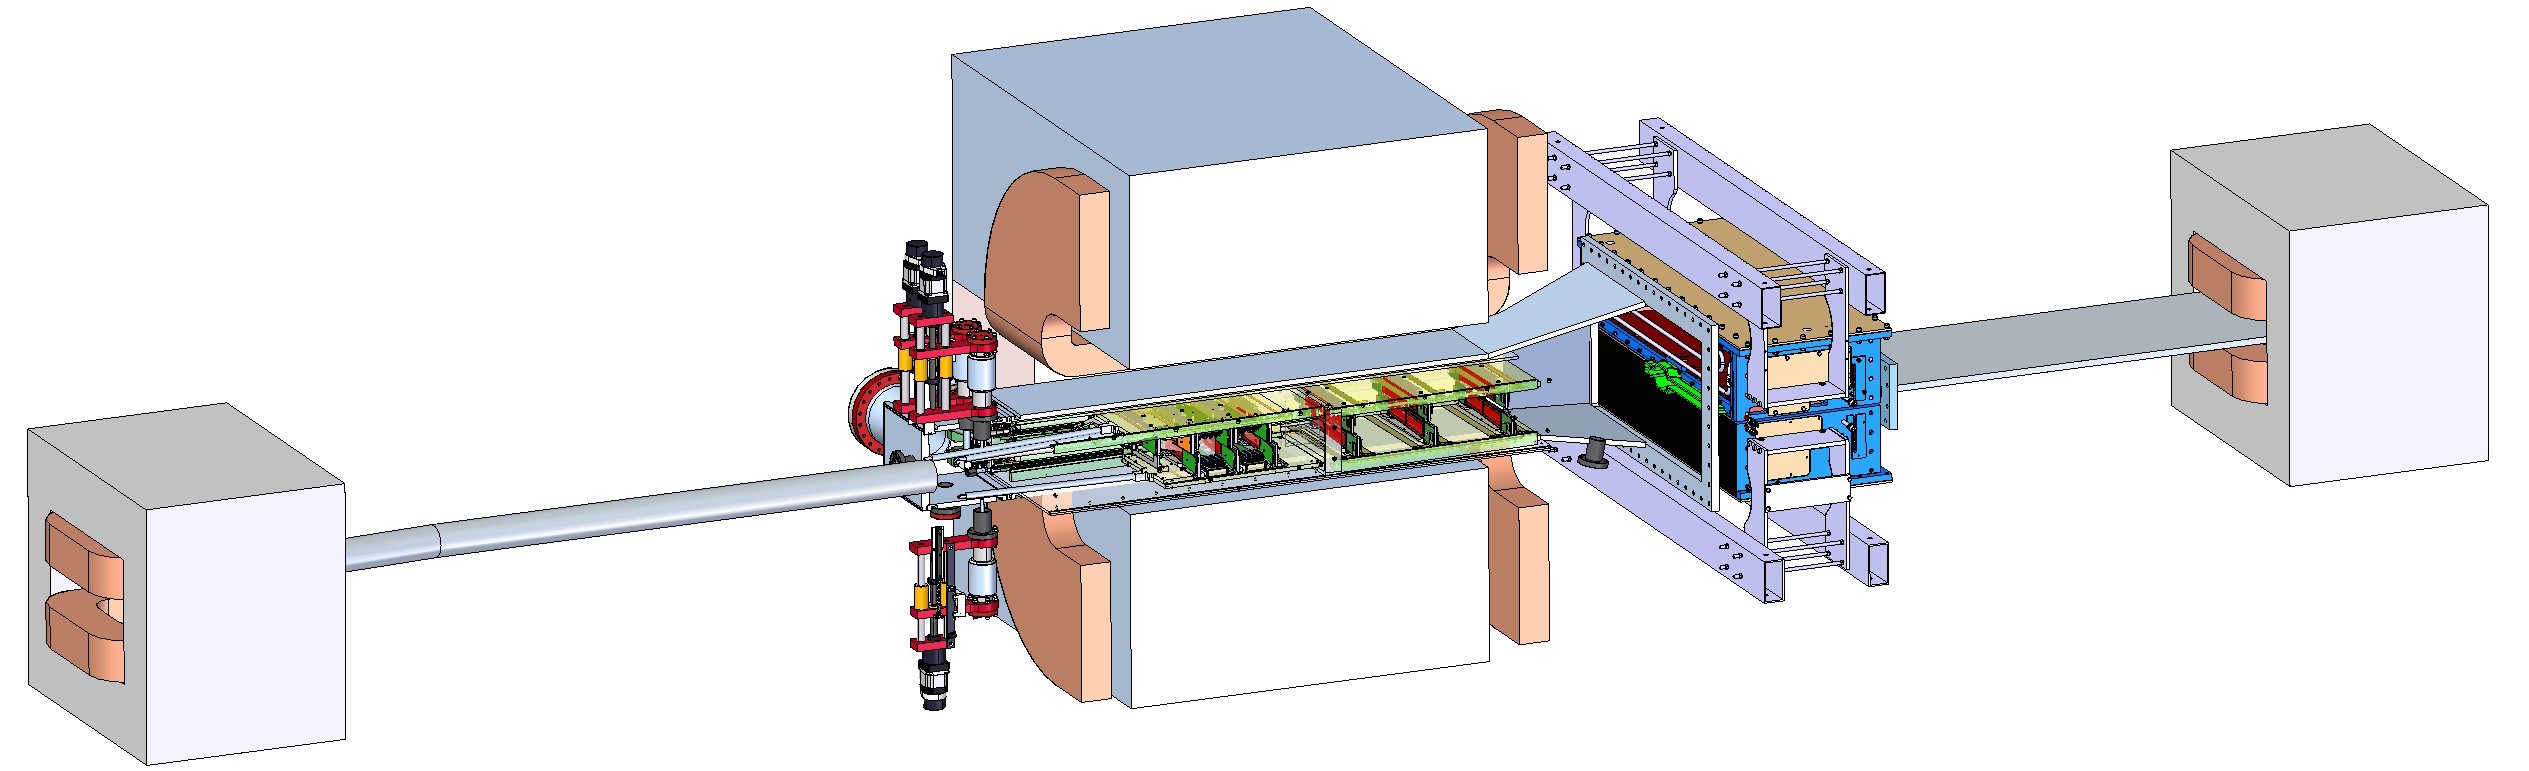
\includegraphics[width=\textwidth]{detector/figs/HPS-pic}
    \caption{View of the HPS setup.}
    \label{fig:hps-pic}
\end{figure}

\begin{figure}[ht]
    \begin{center}
        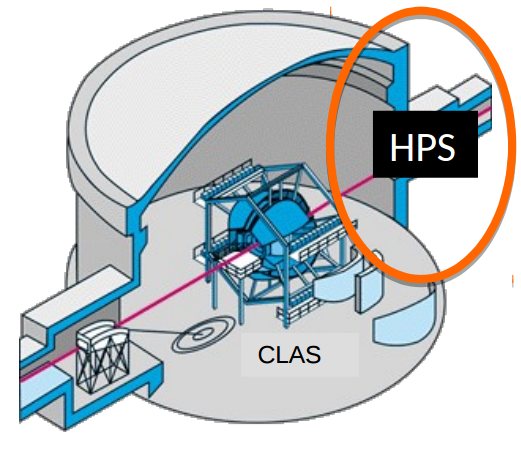
\includegraphics[width=0.5\textwidth]{detector/figs/hallb}
    \end{center}
    \caption{Location of the HPS setup in Hall B.}
    \label{fig:hallb}
\end{figure}

\section{Beamline}

HPS uses the CEBAF (Continuous Electron Beam Accelerator Facility) accelerator at Jefferson Lab (Figure \ref{fig:cebaf}).
CEBAF is a recirculating linac, where the electron beam can take multiple passes through the same set of accelerating cavities.
%CEBAF has a continuous duty cycle because it uses superconducting accelerating cavities, which can be operated continuously without 
The superconducting RF cavities used at CEBAF allow a continuous duty cycle, where beam bunches pass through the accelerator at 1500 MHz without interruption.
A system of RF separators delivers beam to each of four experimental halls at 250 or 500 MHz, and allows each hall to select its own beam energy.
HPS is installed in Hall B, in the downstream alcove of the hall (see Figure \ref{fig:hallb}).

The injector energy is 100 MeV and one pass through the linacs adds 2.2 GeV to the beam energy, so in normal operation, the available beam energies at Hall B are 100 MeV + $n*2.2$ GeV where $n$ is 1 through 5.
During the 2015 engineering run, a mechanical problem disabled one of the two CEBAF helium liquifiers.
With half the cooling power, the superconducting cavities could only be run at half the nominal gradient.
HPS took the opportunity to run at 1.056 GeV, an energy that is not normally available.

HPS relies on the continuous beam structure at CEBAF to reduce pileup.
A beam bunch arrives at HPS every 2 ns, which is comparable to the time resolution of the detectors.
This means that beam backgrounds are spread in time as uniformly as possible.
A larger bunch spacing or lower duty cycle would increase the amount of beam background that overlaps an event of interest.


\begin{figure}[ht]
    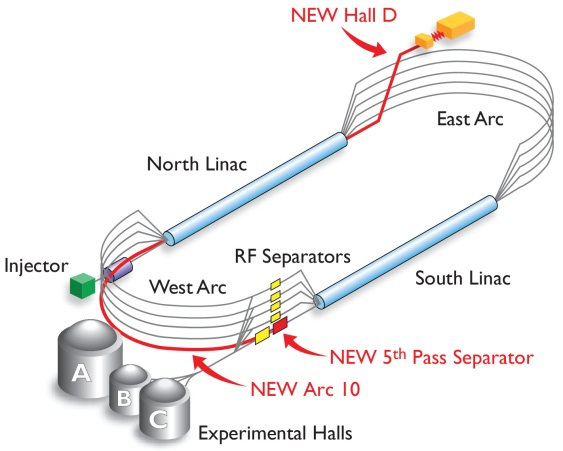
\includegraphics[width=0.6\textwidth]{detector/figs/cebaf}
    \caption{Schematic of the CEBAF accelerator, highlighting components added for the 12 GeV upgrade.}
    \label{fig:cebaf}
\end{figure}

target

beam quality

beam diagnostics

protection

\section{Silicon Vertex Tracker}
\begin{figure}[ht]
    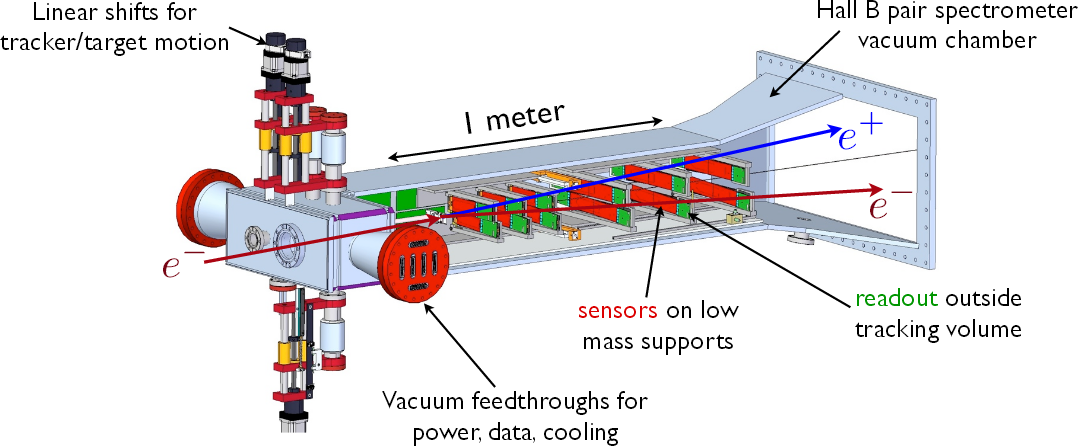
\includegraphics[width=\textwidth]{detector/figs/svt_cutaway}
    \caption{Schematic of the SVT and its support systems.}
    \label{fig:svt-schematic}
\end{figure}

\begin{figure}[ht]
    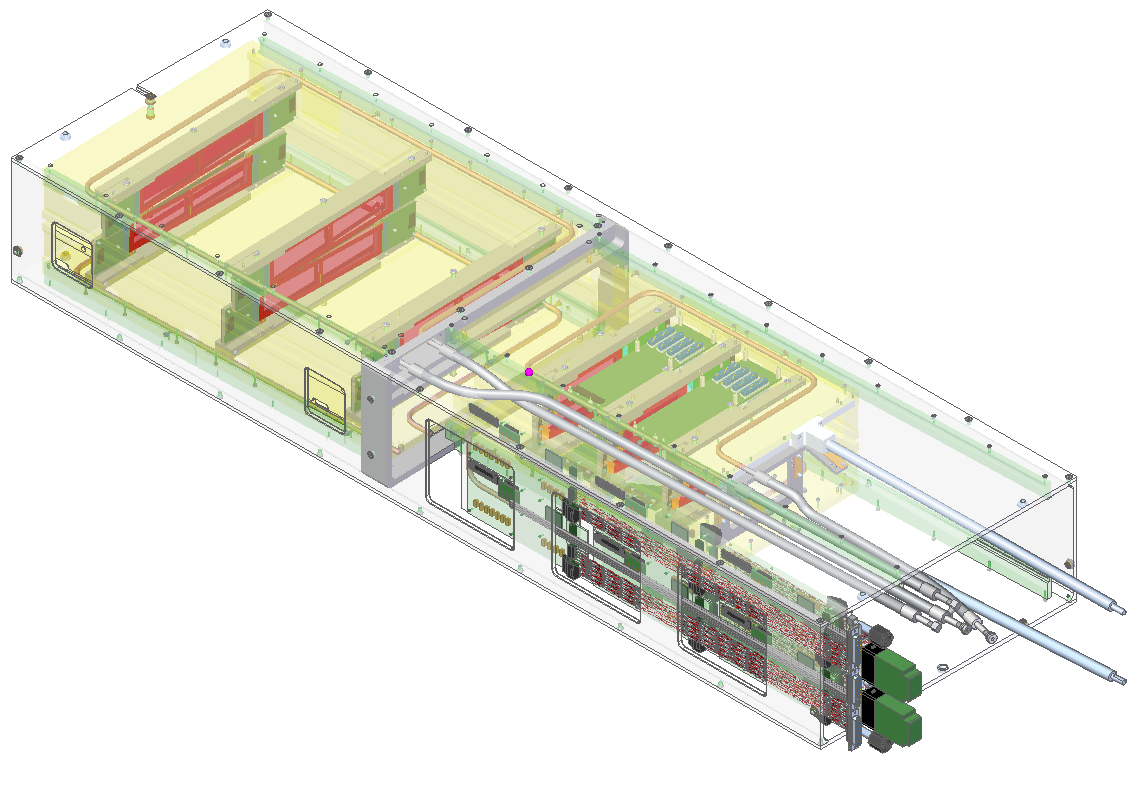
\includegraphics[width=\textwidth]{detector/figs/svt_drawing}
    \caption{Rendering of the SVT as built, showing cooling lines and motion levers.}
    \label{fig:svt-drawing}
\end{figure}

\begin{figure}[ht]
    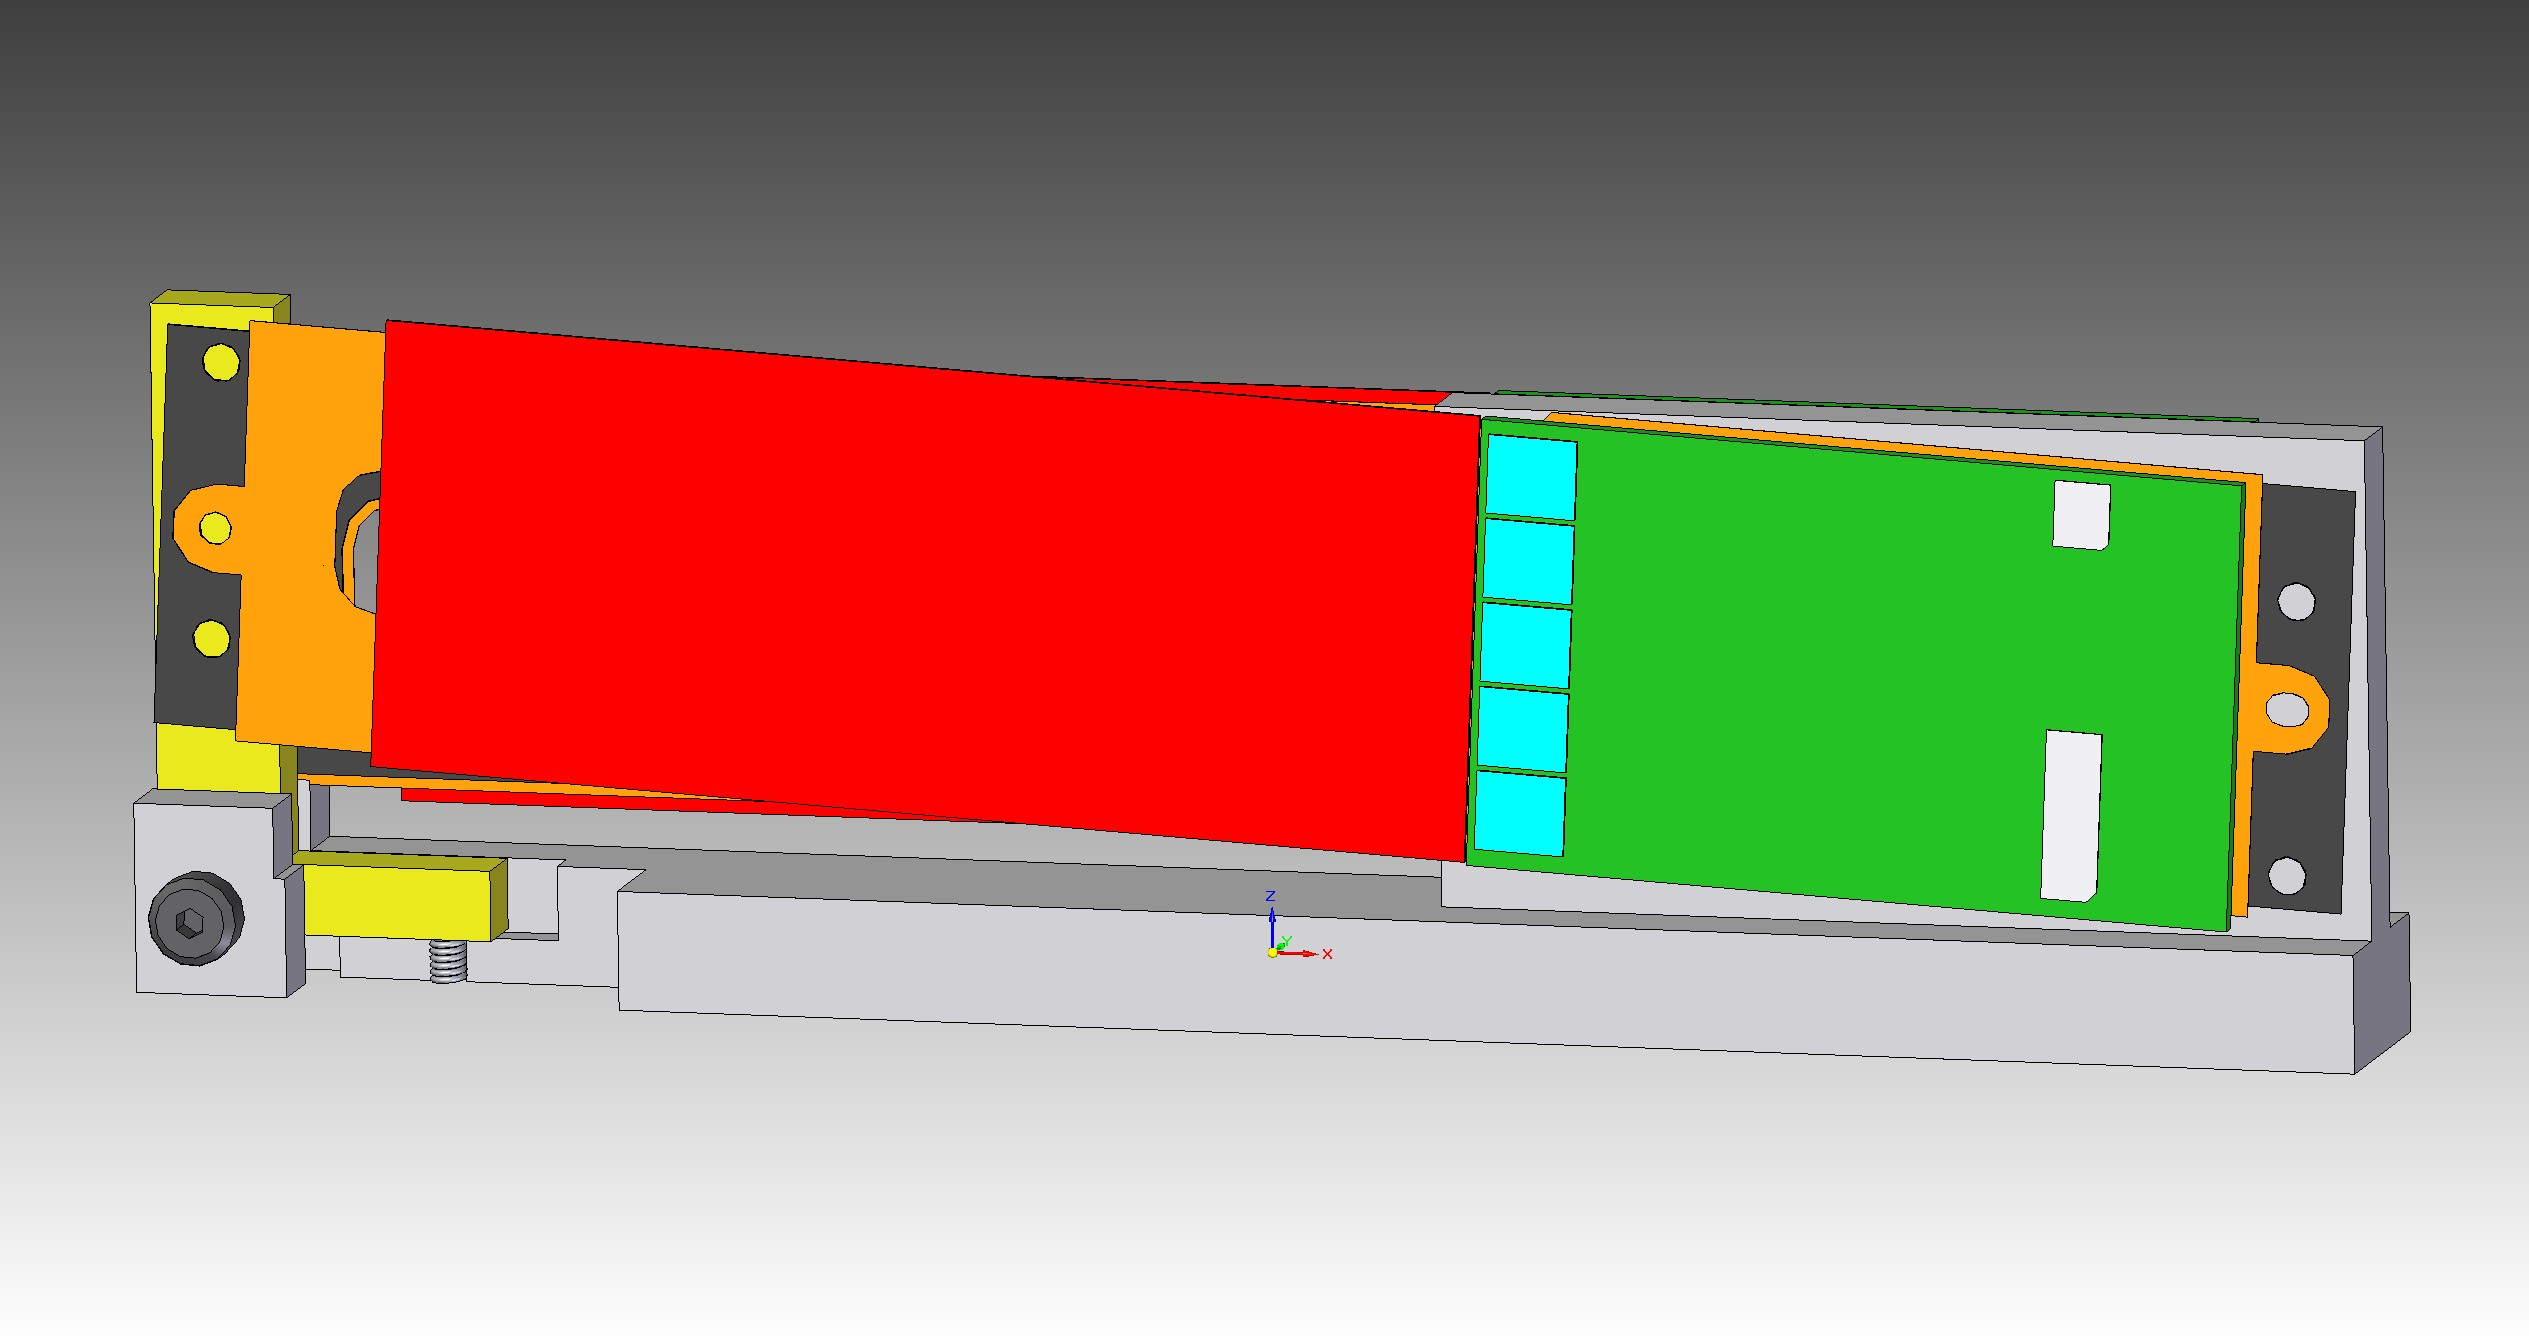
\includegraphics[width=0.5\textwidth]{detector/figs/svt_l123_drawing}
    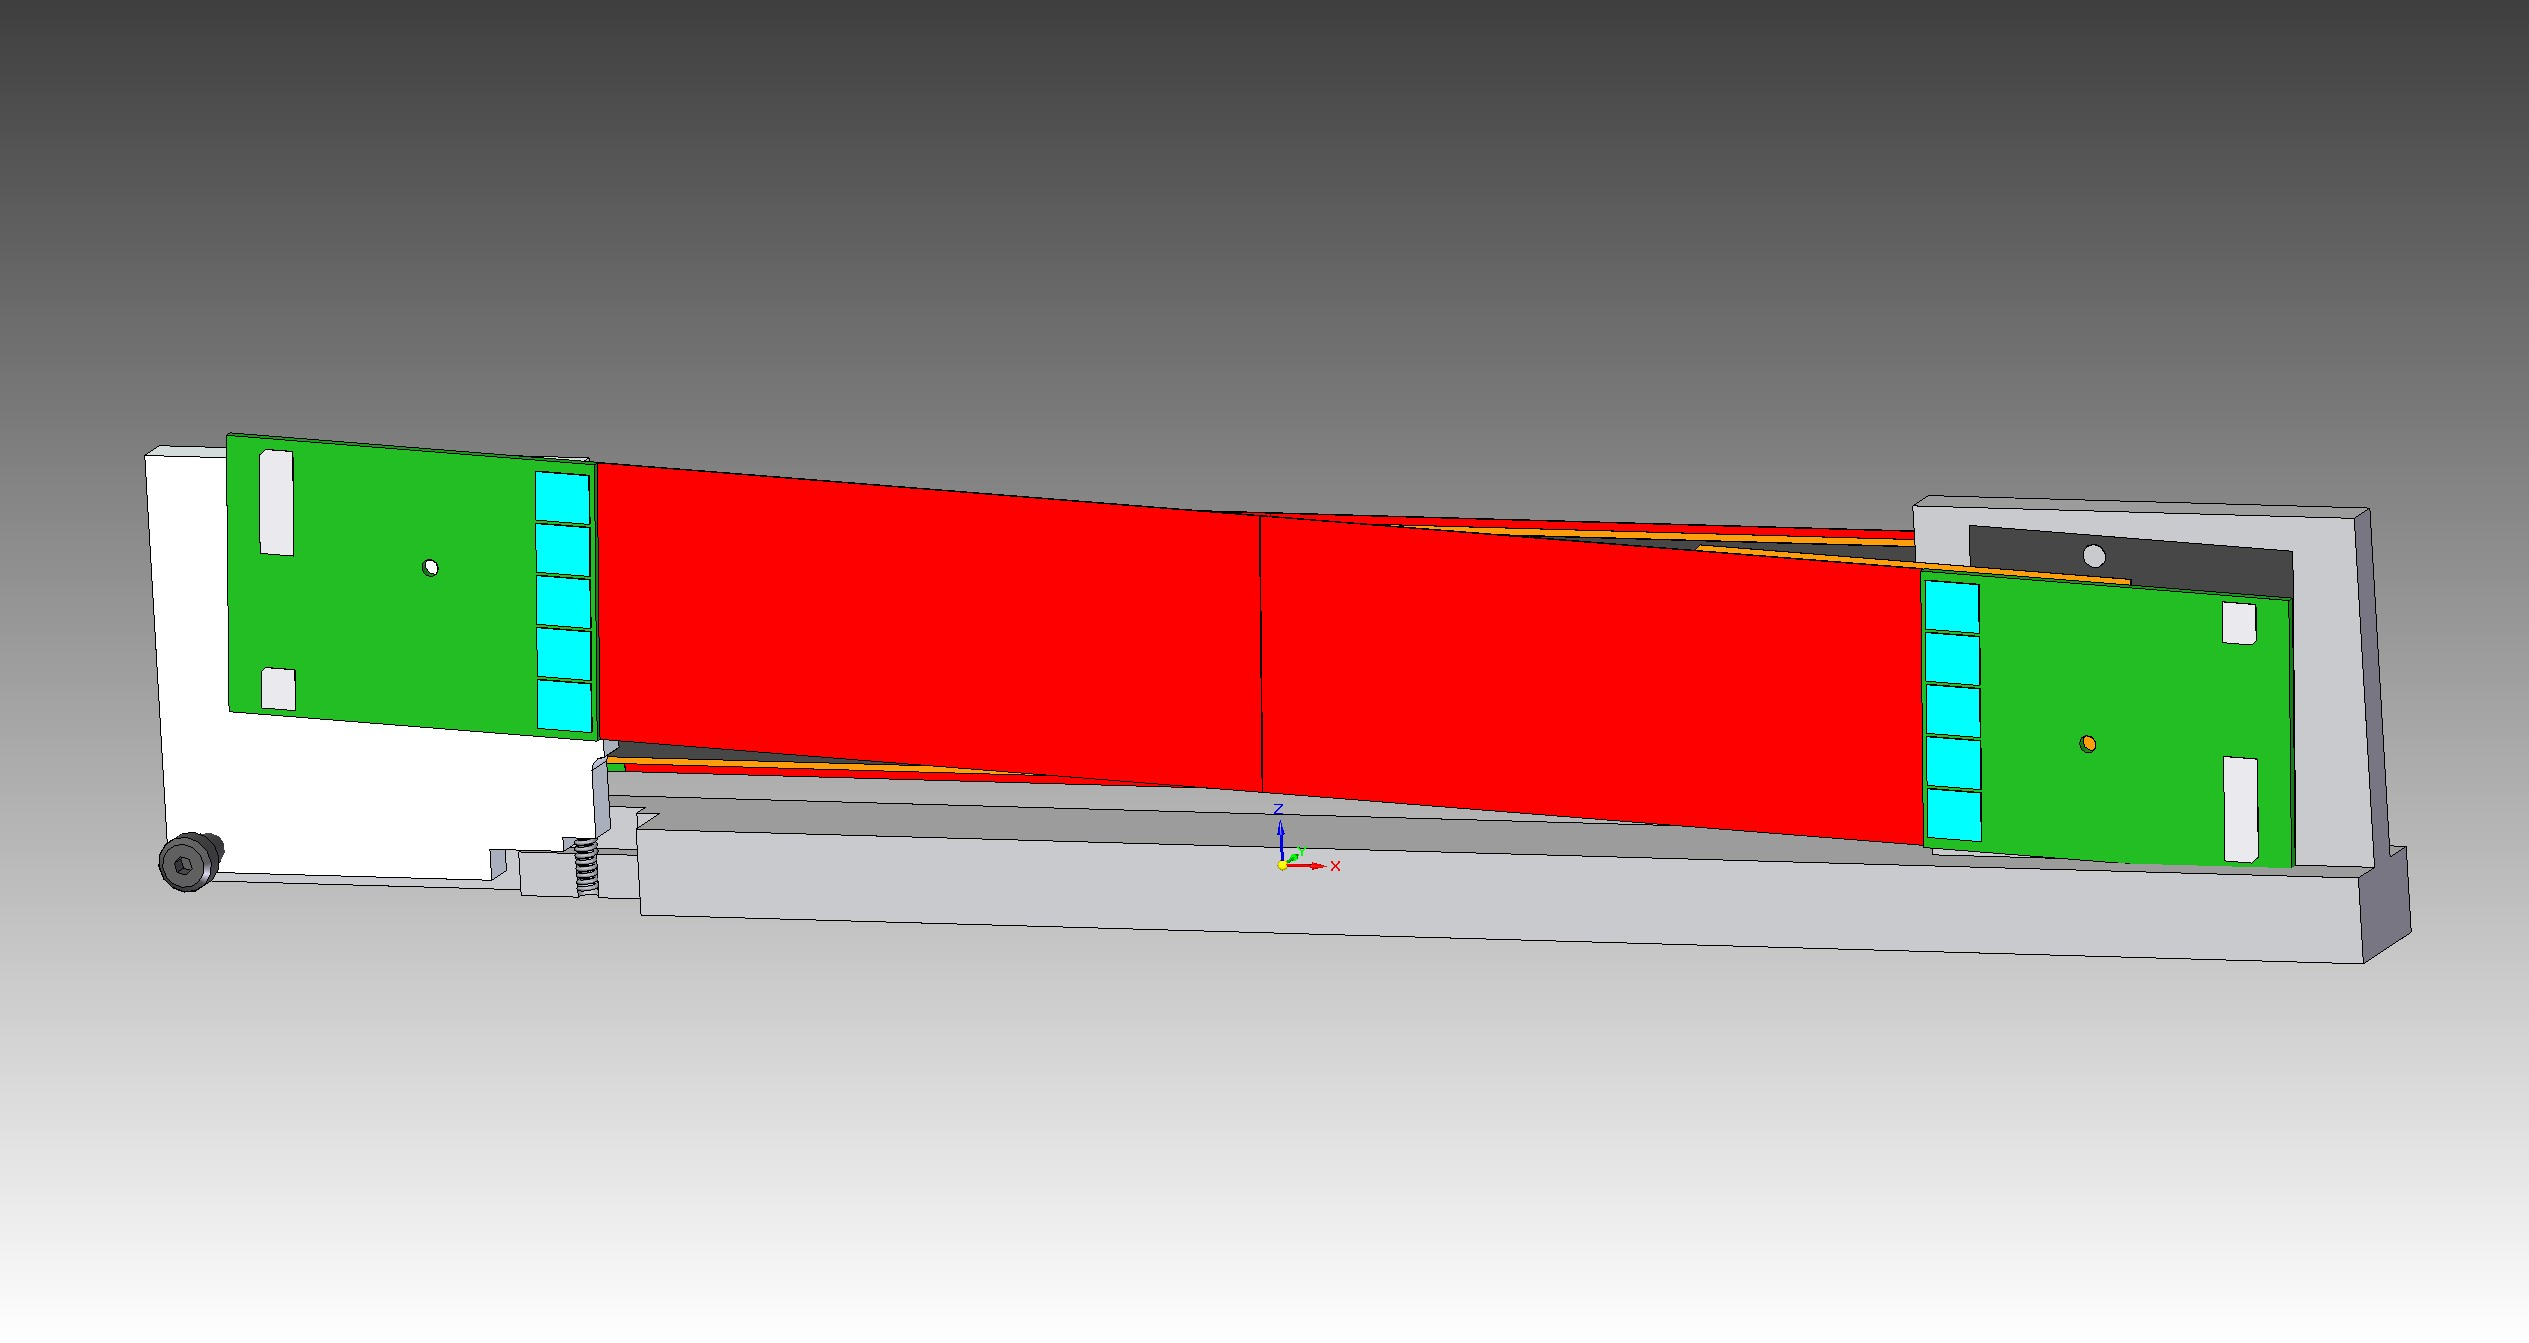
\includegraphics[width=0.5\textwidth]{detector/figs/svt_l456_drawing}
    \caption{Renderings of the L1-3 (left) and L4-6 (right) module designs, with cutaways to show the spring pivots that hold the silicon under constant tension.}
    \label{fig:svt-module-drawing}
\end{figure}

\begin{figure}[ht]
    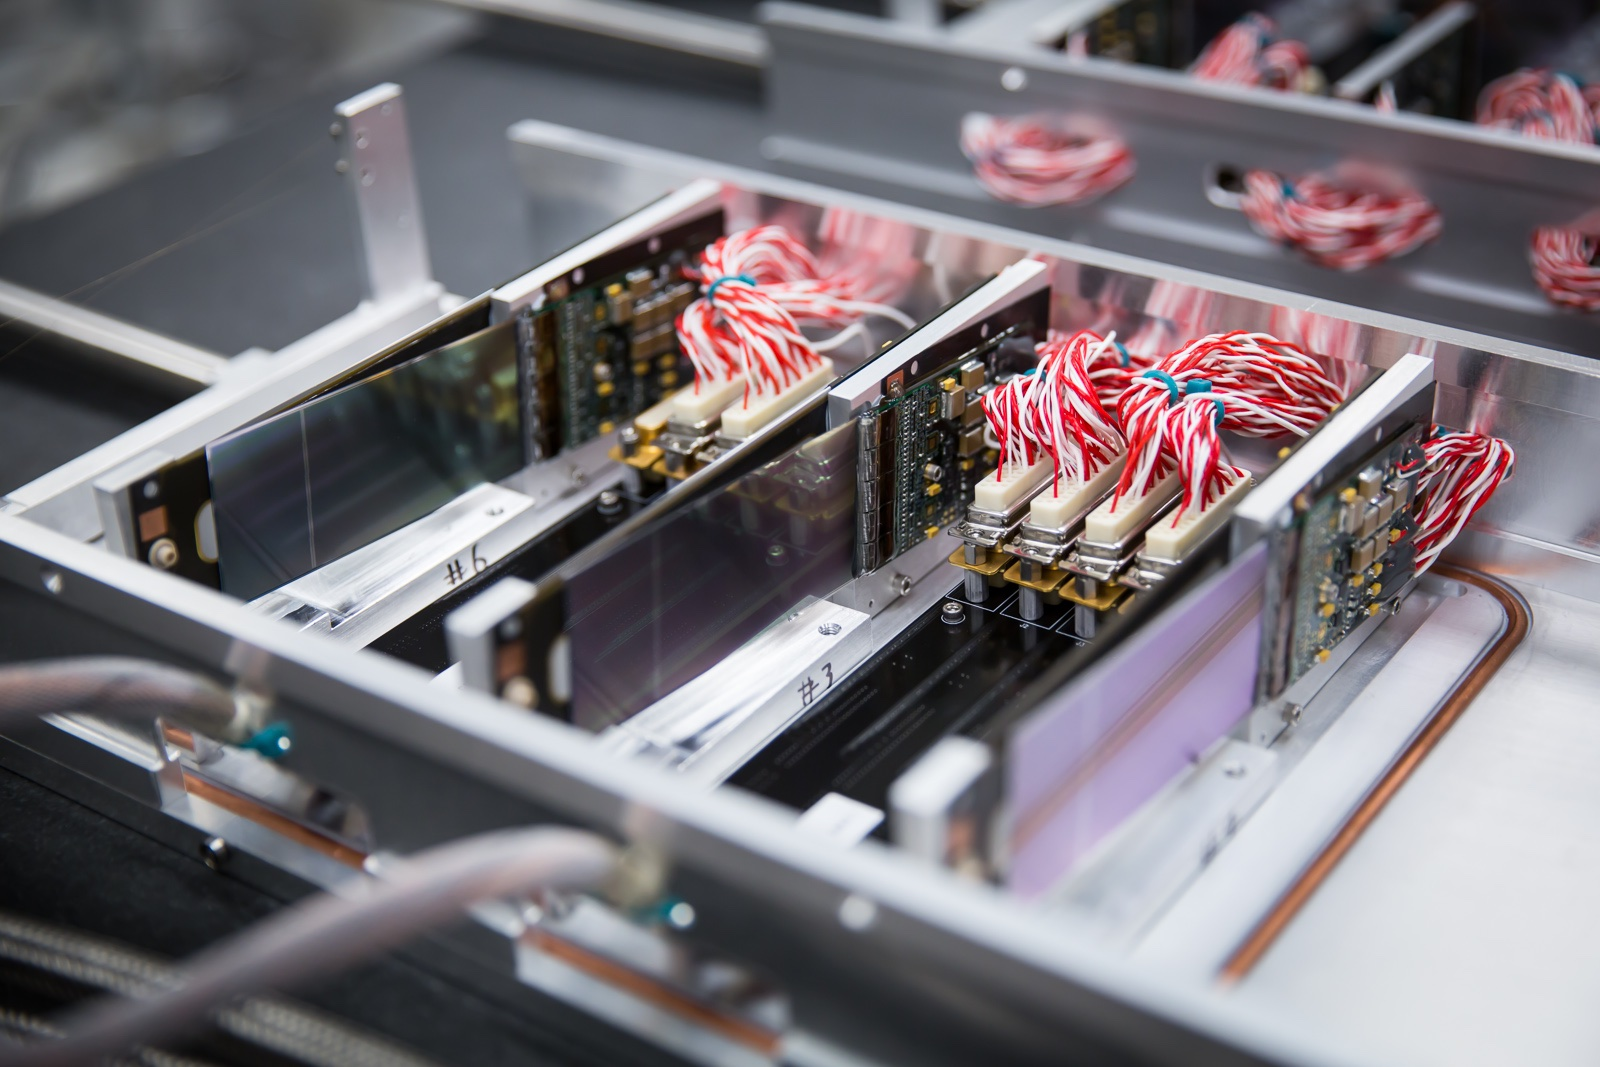
\includegraphics[width=\textwidth]{detector/figs/l123}
    \caption{One of two U-channels for L1-3, fully assembled.}
    \label{fig:l123}
\end{figure}

\begin{figure}[ht]
    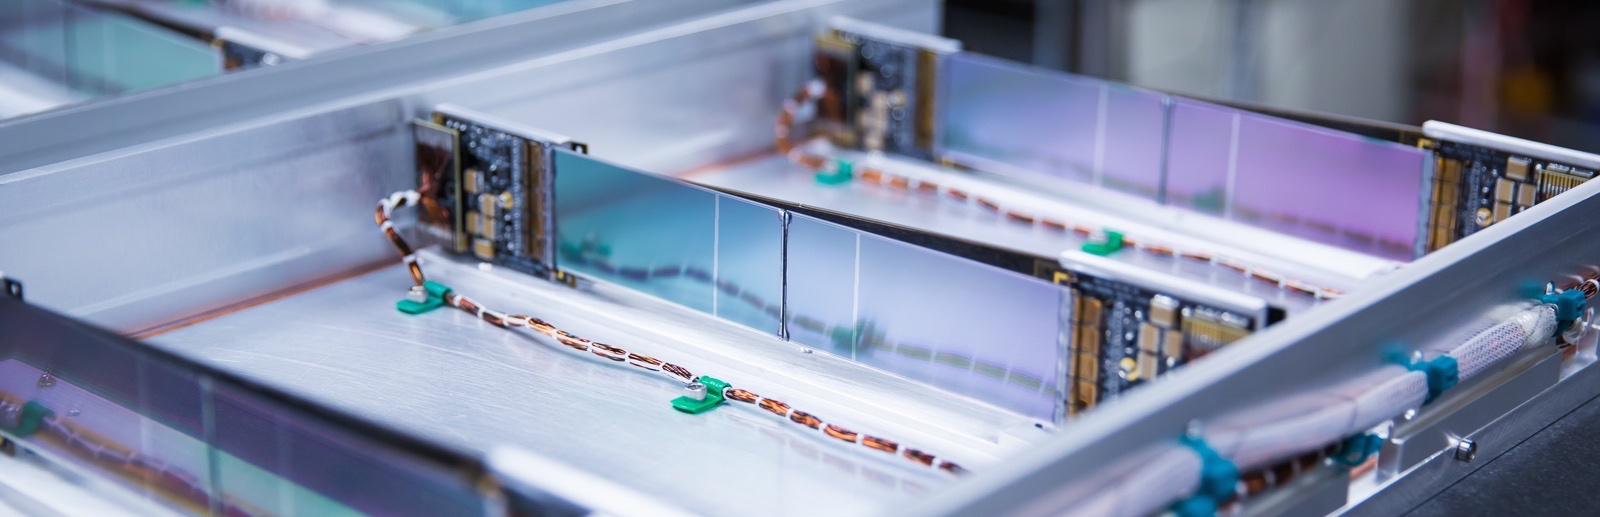
\includegraphics[width=\textwidth]{detector/figs/l456}
    \caption{One of two U-channels for L4-6, fully assembled.}
    \label{fig:l456}
\end{figure}

\begin{figure}[ht]
    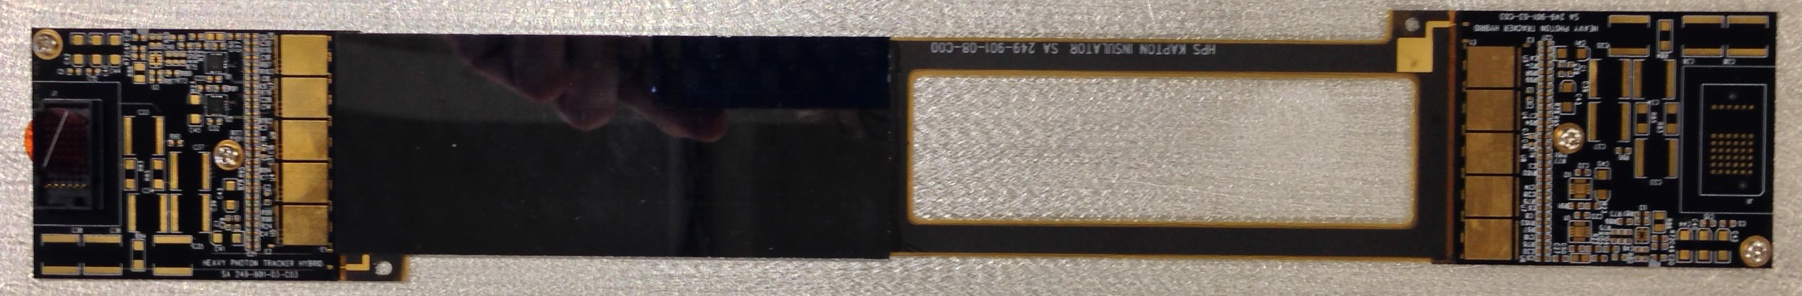
\includegraphics[width=\textwidth]{detector/figs/l456_hm}
    \caption{One half-module for L4-6. The two hybrids (without readout chips, which would be mounted on the gold pads) are at the left and right ends. One sensor is in place, on the left. The carbon fiber support and Kapton passivation layer are visible on the right.}
    \label{fig:l456_hm}
\end{figure}

\begin{figure}[ht]
    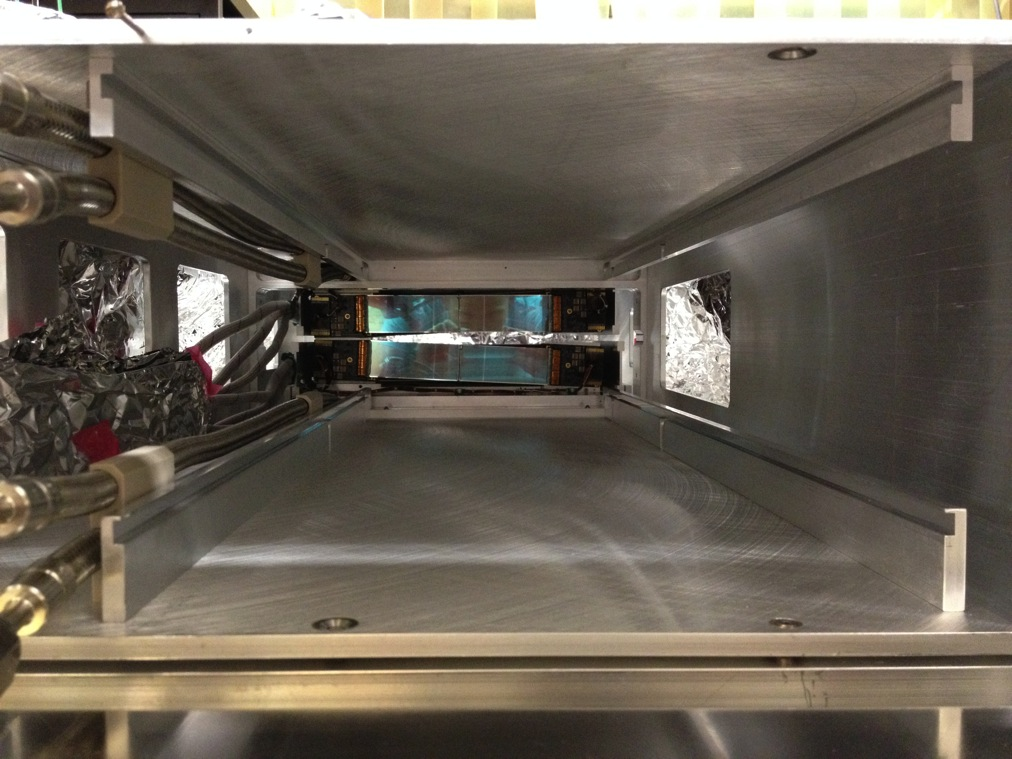
\includegraphics[angle=90,width=\textwidth]{detector/figs/drawers}
    \caption{Inside the SVT box, looking downstream. The L4-6 U-channels are installed. The rails for the L1-3 U-channels can be seen at the top and bottom. When the U-channels are installed, bearings on the U-channels roll along the horizontal slots until they drop down into the vertical slots, guiding the U-channel onto its kinematic mounts.}
    \label{fig:drawers}
\end{figure}

\begin{figure}[ht]
    %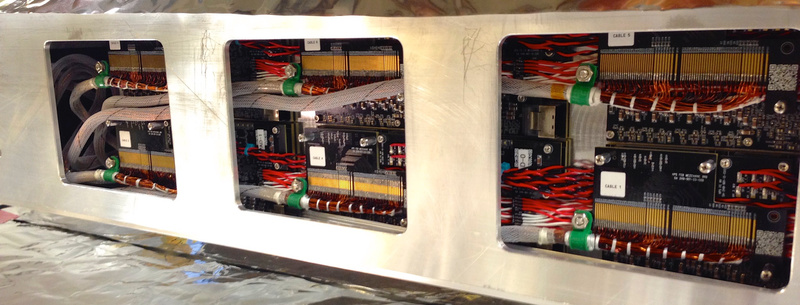
\includegraphics[width=\textwidth]{detector/figs/svt_febs}
    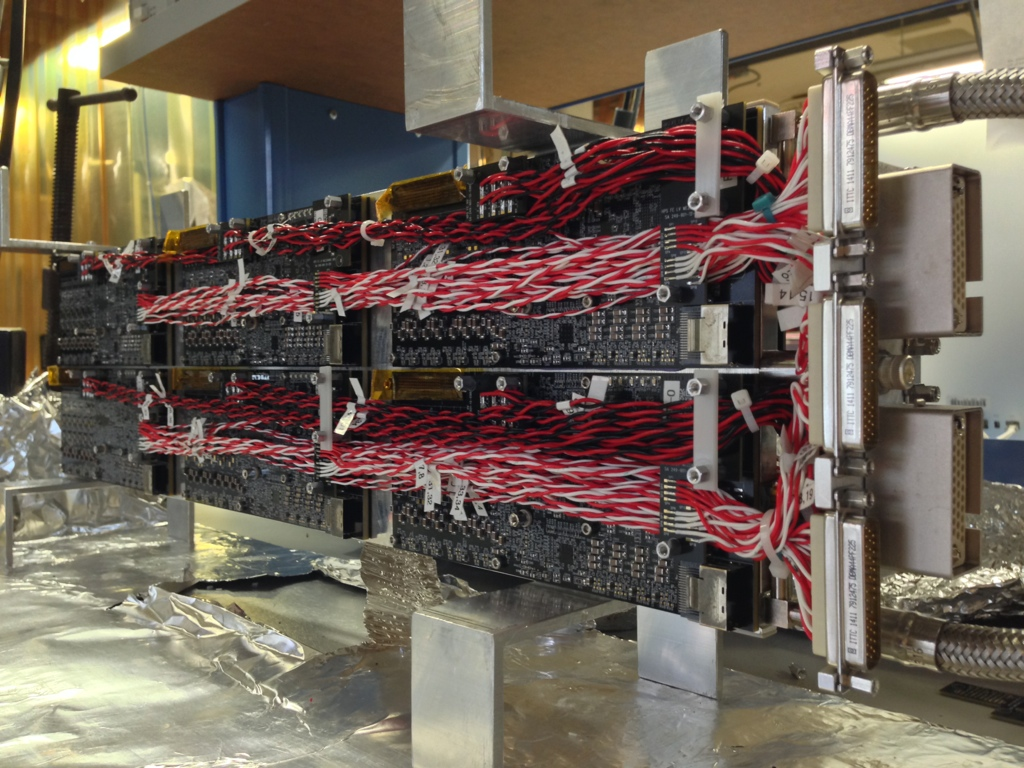
\includegraphics[width=\textwidth]{detector/figs/febplate}
    \caption{The SVT FEBs (frontend boards), mounted on their cooling plate. The red-and-white cables distribute low-voltage power to the FEBs; the red-and-black cables distribute high-voltage bias to the FEBs. The connectors for hybrid power, bias and data are covered with yellow Kapton tape.}
    \label{fig:febplate}
\end{figure}

\begin{figure}[ht]
    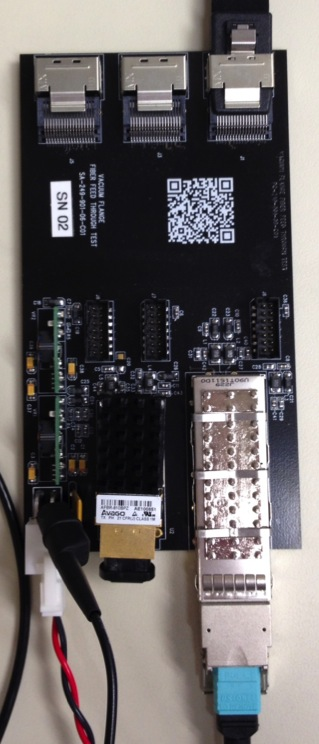
\includegraphics[angle=90,width=\textwidth]{detector/figs/flangeboard}
    \caption{One HPS flange board. The left side of the board operates in vacuum, and has three electrical connectors for high-speed data cables, which connect to the FEBs. The right side of the board operates in air, and has two multi-fiber connectors for data and control signals.}
    \label{fig:flangeboard}
\end{figure}

\begin{figure}[ht]
    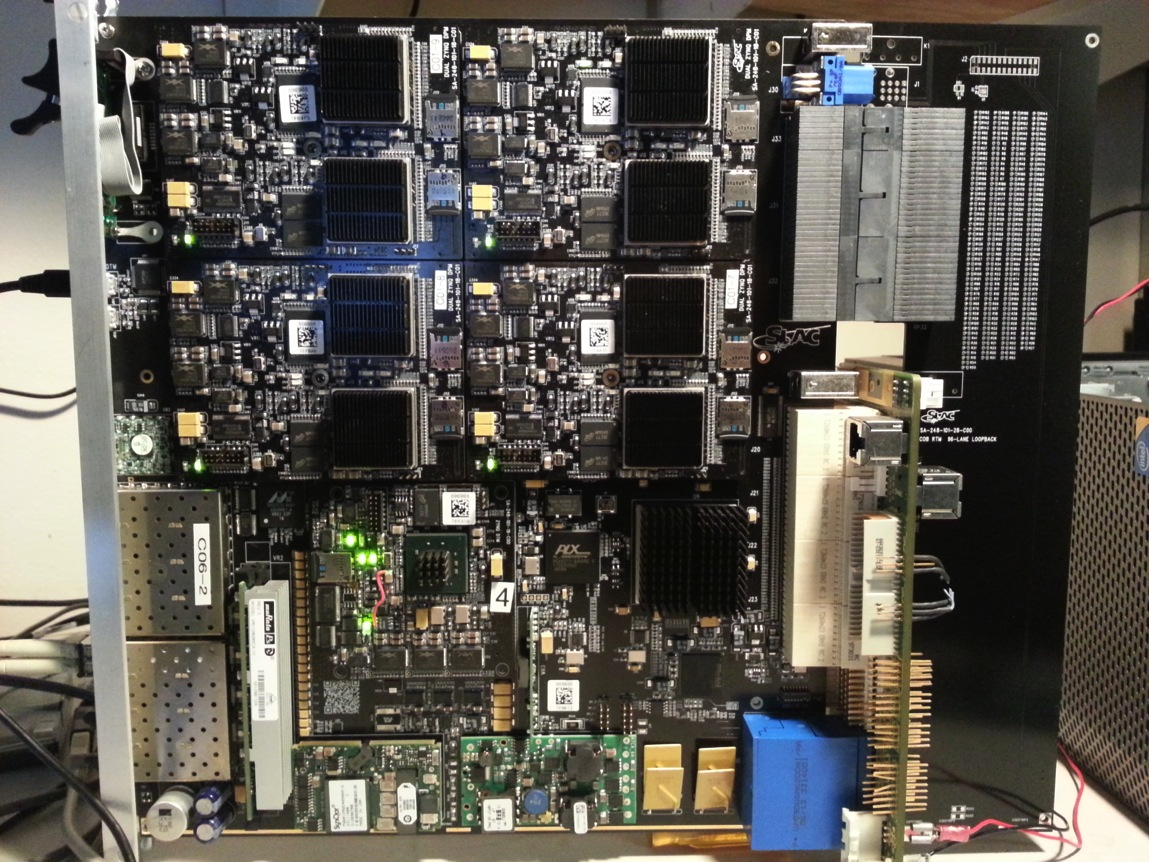
\includegraphics[width=\textwidth]{detector/figs/rce}
    \caption{The RCE system. The COB (Cluster On Board) on the left hosts four RCE (Reconfigurable Cluster Element) daughterboards, which perform the data processing. The RTM (Rear Transition Module) on the right interfaces with fibers carrying data from the flange boards. The COB and RTM would normally be slotted in an ATCA chassis.}
    \label{fig:rce}
\end{figure}


\section{Electromagnetic Calorimeter}
\begin{figure}[ht]
    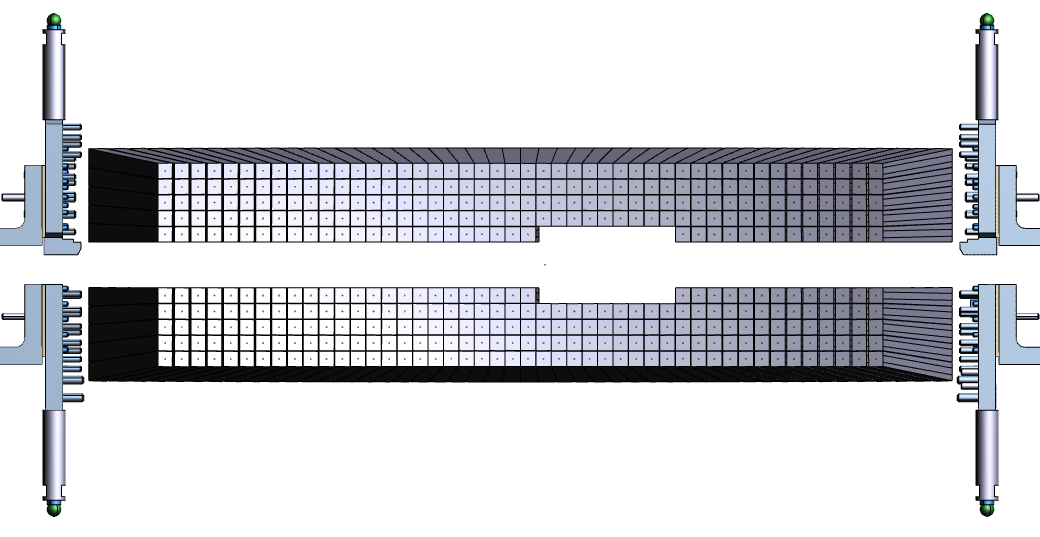
\includegraphics[width=\textwidth]{detector/figs/ECal}
    \caption{Beam's-eye-view of the ECal.}
    \label{fig:ecal}
\end{figure}

\begin{figure}[ht]
    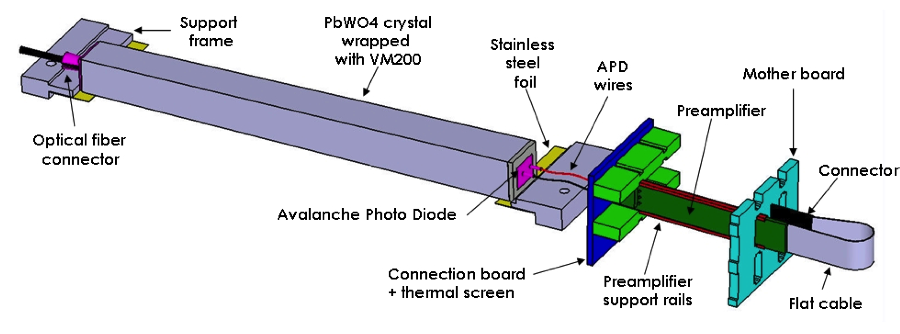
\includegraphics[width=\textwidth]{detector/figs/ecal_module}
    \caption{One ECal crystal with its readout electronics. The optical fiber was used in the CLAS IC for calibration and monitoring, but was removed for HPS. HPS uses LEDs mounted directly in front of the crystals.}
    \label{fig:ecal_module}
\end{figure}

